\documentclass[12pt]{article}

\usepackage[margin=1in]{geometry}
\usepackage[pdftex]{hyperref}
\usepackage{amsmath,amsthm,amssymb,caption,graphicx,mathtools,hyperref,enumerate,enumitem}
\usepackage{centernot}
\usepackage{mdframed,cleveref}
\usepackage{bbm}
\usepackage[makeroom]{cancel}

\usepackage{pgf,tikz-cd,pgfplots}
\pgfplotsset{compat=1.15}
\usepackage{mathrsfs}
\usetikzlibrary{arrows}

\usepackage{multicol}

\usepackage{chngcntr}
\counterwithin{figure}{section}
\numberwithin{equation}{section}

\newtheoremstyle{break}% name
{}%         Space above, empty = `usual value'
{}%         Space below
{}% Body font
{}%         Indent amount (empty = no indent, \parindent = para indent)
{\bfseries}% Thm head font
{}%        Punctuation after thm head
{\newline}% Space after thm head: \newline = linebreak
{#1 #2 \normalfont #3}%         Thm head spec

\theoremstyle{definition}
\newtheorem*{remark}{Remark}

\theoremstyle{definition}
\newtheorem*{definition}{Definition}

\theoremstyle{definition}
\newtheorem*{theorem}{Theorem}

\theoremstyle{definition}
\newtheorem*{corollary}{Corollary}

\theoremstyle{break}
\newtheorem*{example}{Example}

\theoremstyle{definition}
\newtheorem*{lemma}{Lemma}

\theoremstyle{definition}
\newtheorem*{objective}{Objective}

\newmdenv[leftline=false,topline=false]{topright}
\let\proof\relax
\usepackage[utf8]{inputenc}
\usetikzlibrary{positioning}
\newcommand{\n}{\mathbb{N}}
\newcommand{\z}{\mathbb{Z}}
\newcommand{\q}{\mathbb{Q}}
\newcommand{\cx}{\mathbb{C}}
\newcommand{\real}{\mathbb{R}}
\newcommand{\E}{\mathbb{E}}
\newcommand{\V}{\mathbb{V}}
\newcommand{\divs}{\,\big|\,} %divides (a|b)
\newcommand{\bb}[1]{\mathbb{#1}}
\let\k\relax
\newcommand{\k}{\mathbf{k}}
\newcommand{\ita}[1]{\textit{#1}}
\newcommand\inv[1]{#1^{-1}}
\newcommand\setb[1]{\left\{#1\right\}}
\newcommand{\vbrack}[1]{\langle #1\rangle}
\newcommand{\determinant}[1]{\begin{vmatrix}#1\end{vmatrix}}
\newcommand{\abs}[1]{\left\vert #1 \right\vert}
\newcommand{\norm}[1]{\left\lVert#1\right\rVert}
\DeclareMathOperator{\Id}{Id}


\hypersetup{
	colorlinks,
	linkcolor=blue
}

\usepackage{tocloft} %table of contents package
\renewcommand{\cftsecleader}{\cftdotfill{\cftdotsep}}
\newcommand{\atoc}[1]{\addtocontents{toc}{#1\par}}

\setlength{\parindent}{0pt}

\title{Numerical Methods for Differential Equations}
\author{Ferran Arqué}
\date{2018}

\begin{document}

\maketitle

\tableofcontents

\atoc{\hyperref[sec:ode]{\color{black}\textbf{Ordinary Differential Equations}}}

\newpage
\section*{}\label{sec:ode}
\vspace*{\fill}
\hspace*{\fill}
\huge{ORDINARY DIFFERENTIAL EQUATIONS}
\hspace*{\fill}
\vspace*{\fill}
\normalsize
\newpage
\section{Ordinary Differential Equations. Basic concepts}

\subsection{Introduction and some notation}

Given $y' = f(x,y)$, where $\begin{cases} y(x) \in \real^n\\ f:\real\times\real^n \to \real^n\end{cases}$

\begin{definition}
  We denote by $y(x)$ the exact solution of the ODE system above.
\end{definition}

\begin{definition}
  $y_k$ is the approximation of $y(x_k)$ (after $k$ steps).
\end{definition}

\begin{objective}
  We want to approximate $y(x)$ within a given interval $[x_0, x_n]$. \\
  \footnotesize{
  \begin{multicols}{3}
    We know $\begin{cases}x_0\\x_1\\x_2\\\vdots\\x_n \end{cases}$\\
    \-\hspace{-2cm}We'd like to know $\begin{cases}y(x_0)\\y(x_1)\\y(x_2)\\\vdots \\y(x_n) \end{cases}$\\
    \-\hspace{-2cm}We find $\begin{cases} y_0\\y_1\\y_2\\\vdots \\y_n \end{cases}$ (given by a method)
  \end{multicols}
  }
\end{objective}
\normalsize
\begin{definition}
  $\norm{y(x_n) - y_n}$ is the \textbf{global error}.
\end{definition}

\begin{definition}
  We define the \textbf{local truncation error} as the error caused by one iteration, i.e. $$LTE = \norm{y(x_k) - y_k} \qquad \text{\big(assuming the \textit{localizing assumption}: $y_{k-1} = y(x_{k-1})$\big)}$$
\end{definition}

\begin{definition}
  A method is of \textbf{order} $p$ if the LTE is of the form $$\text{LTE} = Ch^{p+1} + \mathcal{O}(h^{p+2})$$
\end{definition}

\subsection{Euler's method}
\subsubsection{Formulation}
Consider the differential equation system
\begin{equation}\label{sys1.2}
  y'(x) = f(y(x)), \qquad y(x_0) = y_0 \qquad (\text{with } f:\real^n \to \real^n)
\end{equation}

We'll also assume, for later results, that $f$ satisfies a Lipschitz condition $$\norm{f(y) - f(z)} \leq L\norm{y-z}$$

Now, we want to find an approximation of (\ref{sys1.2}) on an interval $[x_0, x_N]$, so we'll create a set of $N+1$ evenly spaced points between $x_0$ and $x_N$, where $N$ is the number of steps and $h = \dfrac{x_N-x_0}{N}$ the stepsize.\\

To do that, we can use Euler's method
\[
  y_{n+1} = y_n + hf(y_n)
\]

\newpage

\subsubsection{Local truncation error}

We want to find $LTE = \norm{y(x_{n+1}) - y_{n+1}}$. Let's expand it

\begin{align*}
    y(x_{n+1}) - y_{n+1} &= y(x_n + h) - y_{n+1} = y(x_n) + hy'(x_n) + \mathcal{O}(h^2) - y_n - hf(y_n) \underset{\text{Loc.ass.}}{=} \\
    &= y(x_n)+ hy'(x_n) + \mathcal{O}(h^2) - y(x_n) - hf(y_{x_n}) \\
    &= hy'(x_n) + \mathcal{O}(h^2) - hy'(x_n) = \mathcal{O}(h^2)
\end{align*}
  
So LTE = $\mathcal{O}(h^2)$, and the method has order $p=1$.

\subsubsection{Convergence}

For the method to be convergent, it has to verify $$\norm{y(x_N) - y_N} \underset{h\to0}{\longrightarrow} 0$$

Similar as what we did with the LTE, we'll find a bound for the error in one step, but this time without using the localizing assumption:

\begin{align*}
    \norm{y(x_{n+1}) - y_{n+1}} &= \norm{y(x_n + h) - y_n - hf(y_n)} \underset{\text{Taylor}}{=} ||y(x_n) + h\underbrace{y'(x_n)}_{f(y(x_n))} + \Tilde{c}h^2 - y_n - hf(y_n)|| \\
    &\leq \norm{y(x_n) - y_n} + h\underbrace{\norm{f(y(x_n)) - f(y_n)}}_{\substack{\text{\rotatebox{270}{$\leq$}} \\ L\norm{y(x_n) - y_n}}} + ch^2 \leq (1+hL)\norm{y(x_n) - y_n} + ch^2 \quad \forall n
\end{align*}

Thus
\begin{align*}
    &\norm{y(x_1) - y_1} \leq (1+hL)\norm{y(x_0) - y_0} + c_1h^2 \\
    &\norm{y(x_2) - y_2} \leq (1+hL)\norm{y(x_1) - y_1} + c_2h^2 \leq (1+hL)^2\norm{y(x_0) - y_0} + (1+hL)c_1h^2 + c_2h^2 \\
    &\norm{y(x_3) - y_3} \leq (1+hL)^3\norm{y(x_0) - y_0} + (1+hL)^2c_1h^2 + (1+hL)c_2h^2 + c_3h^2\\
    &\hspace{1.2cm}\vdots
\end{align*}
%\-\\
Let $C = \underset{i}{\text{max}}\,c_i$ \\

Then
\begin{align*}
    \norm{y(x_N) - y_N} \leq (1+hL)^N \norm{y(x_0) - y_0} + \underbrace{\Big(1 + (1+hL) + (1+hL)^2 + \ldots + (1+hL)^{N-1}\Big)}_{\substack{\text{\hspace{-0.94cm}geom$\to\,$\rotatebox{90}{$=$}}\\\frac{(1+hL)^N-1}{hL}}}Ch^2
\end{align*}

\[
  \implies \norm{y(x_n) - y_N} \leq (1+hL)^N\underbrace{\norm{y(x_0) - y_0}}_{\substack{\text{\hspace{-0.6cm}(\ref{sys1.2})\,\rotatebox{90}{=}}\\ 0}} + \frac{(1+hL)^N-1}{\cancel{h}L}\cdot Ch^{\cancel{2}} \leq Ah \to 0
\]

\begin{remark}
  In the last inequality we used $(1+hL)^N = e^{N\log(1+hL)} \underset{\substack{\log(1+x)\\\leq x + cx^2}}{=} e^{NhL + \alpha Nh^2} =$ $=e^{L(x_N-x_0)}\cdot e^{ch}\qquad$ ($Nh = x_n-x_0$)
\end{remark}

\newpage

\subsection{Improved Euler's method} \label{imprEu}
\subsubsection{Formulation}
\begin{figure}[h]
    \centering
    \definecolor{zzqqtt}{rgb}{0.6,0.,0.2}
    \definecolor{qqttzz}{rgb}{0.,0.2,0.6}
    \definecolor{qqwwzz}{rgb}{0.,0.4,0.6}
    \definecolor{xdxdff}{rgb}{0.49019607843137253,0.49019607843137253,1.}
    
    \begin{tikzpicture}[line cap=round,line join=round,>=triangle 45,x=0.9285714285714286cm,y=0.9090909090909091cm]
    \begin{axis}[
    x=0.9285714285714286cm,y=0.9090909090909091cm,
    axis lines=middle,
    xmin=-1.0,
    xmax=13.0,
    ymin=-1.0,
    ymax=10.0,
    xtick={-0.0},
    ytick={-0.0},]
    \clip(-1.,-1.) rectangle (13.,10.);
    \draw[line width=1.pt,smooth,samples=100,domain=1.2000000009119923E-2:13.0] plot(\x,{ln((\x)^(5.0))-5.0});
    \draw [->,line width=1.pt,color=qqwwzz] (4.789374476513226,2.831999067204186) -- (9.680475596667712,8.660000685442492);
    \draw [->,line width=1.pt,color=qqwwzz] (4.789374476513226,2.831999067204186) -- (7.261114317049705,5.777205767419718);
    \draw [->,line width=1.pt,color=xdxdff] (7.261114317049705,5.777205767419718) -- (12.459510324028214,8.81562663017468);
    \draw [->,line width=1.pt,color=xdxdff] (4.789374476513226,2.831999067204186) -- (10.,6.);
    \draw [->,line width=1.pt,color=qqttzz] (9.680475596667712,8.660000685442492) -- (10.,6.);
    \draw [->,line width=1.pt,color=qqttzz] (4.789374476513226,2.831999067204186) -- (9.827482089829717,7.436190020287211);
    \draw [->,line width=1.pt,color=zzqqtt] (4.789374476513226,2.831999067204186) -- (7.731770530417767,5.520975629746587);
    \draw (6.279627438393455,6.60187417823135) node[anchor=north west] {$y_{n+1}^*$};
    \draw (4.257396566874901,3.6040056055416194) node[anchor=north west] {$y_n$};
    \draw [color=zzqqtt](7.7,5.5) node[anchor=north west] {$y_{n+1}$};
    \draw (10.714344261899054,9.475570679862926) node[anchor=north west] {$f(y_{n+1}^*)$};
    \draw (11.35294348448386,7.258212268110167) node[anchor=north west] {$y$};
    \draw (8.0,8.8) node[anchor=north west] {$f(y_n)$};
    \begin{scriptsize}
    \draw [fill=xdxdff] (4.789374476513226,2.831999067204186) circle (2.5pt);
    \draw [fill=xdxdff] (7.261114317049705,5.777205767419718) circle (2.5pt);
    \draw [fill=zzqqtt] (7.731770530417767,5.520975629746587) circle (2.5pt);
    \end{scriptsize}
    \end{axis}
    \end{tikzpicture}
    \caption{One step of the enhanced Euler's method}
    \label{fig:EnhancedEuler}
\end{figure}\-\\

Given $y'(x) = f(y(x)), \quad y: \real \to \real, \quad f:\real \to \real$, we'll go through the steps to deduce the improved Euler's method (also called Heun's method) with the help of the scheme in \text{Figure \ref{fig:EnhancedEuler}}. \\

The auxiliary point $y_{n+1}^*$ can be found doing one step of the standard Euler's method, so 

\[
  y_{n+1}^* = y_n + h\cdot f(y_n)
\]
\vspace{0.01cm}

To get the point $y_{n+1}$ we compute the average vector of $f(y_{n+1}^*)$ and $f(y_n)$, and with this new vector, we can apply again a step of Euler's method, ending up with our method

\[
  \boxed{y_{n+1} = y_n + \frac{h}{2}\cdot \left(f(y_{n+1}^*) + f(y_n)\right)}
\]
\newpage

\subsubsection{Local truncation error}

The Local Truncation Error is given by:

\[
  LTE = \norm{\textit{method} - \textit{exact solution}}
\]

Then

\[
  LTE = \norm{y_{n+1} - y(x_{n+1})} = \Big\rVert y_n + \frac{h}{2}f(y_n) + \frac{h}{2}f(y_{n+1}^*) - \underbrace{y(x_{n+1})}_{y(x_n + h)}\Big\rVert = (*)
\]

Applying Taylor on $f(y_{n+1}^*) = f\left(y_n + hf(y_n)\right)$, we have

\[
  f\left(y_n + hf(y_n)\right) = f(y_n) + hf(y_n)f'(y_n) + \mathcal{O}(h^2)
\]
\\
and on $y(x_n +h)$ we have

\[
  y(x_n + h) = y(x_n) + h\cdot y'(x_n) + \frac{h^2}{2}\cdot y''(x_n) + \mathcal{O}(h^3)
\]

(In this case, we expand to second order for later simplifications)

\footnotesize

\[
    (*) = \norm{y_n + \frac{h}{2}f(y_n) + \frac{h}{2}\left(f(y_n) + hf(y_n)f'(y_n) + \mathcal{O}(h^2) \right) - \left(y(x_n) + h\cdot y'(x_n) + \frac{h^2}{2}\cdot y''(x_n) + \mathcal{O}(h^3) \right)} \quad (1)
\]

\normalsize
\-\\
Now, given $y'(x) = f(y(x))$, we have

\vspace{-0.5cm}

\begin{align*}
    y''(x) &= f'(y(x))\cdot y'(x) \\
           &= f'(y(x)) \cdot f(y(x))
\end{align*}

and we can rewrite the following expression as:

\[
  \frac{h^2}{2}f(y(x))f'(y(x)) = \frac{h^2}{2}y''(x)
\]

With that and the localising assumption ($y_n = y(x_n)$), we can simplify most of the terms in (1) and we end up with

\small

\[
  \norm{\cancel{y_n} + \bcancel{\frac{h}{2}f(y_n) + \frac{h}{2}f(y_n)} + \xcancel{\frac{h^2}{2}f(y_n)f'(y_n)} + \mathcal{O}(h^3)  - \left(\cancel{y(x_n)} + \bcancel{h\cdot y'(x_n)} + \xcancel{\frac{h^2}{2}\cdot y''(x_n)} + \mathcal{O}(h^3) \right)} = \mathcal{O}(h^3)
\]

\normalsize
\-\\\\
So LTE $= \mathcal{O}(h^3)$\\

\begin{remark}
  Of course, this method also works for $y: \real \to \mathbb{R}^n, \, f:\real^n \to \real^n$
\end{remark}

\subsection{Final remarks}
\begin{itemize}
    \item There's an enhanced Euler's method of order $2$ similar to the previous one: $$\boxed{y_{n+1} = y_n + hf\left(\frac{y_{n+1}^* + y_n}{2}\right)}$$
    \item If we have a method of order $\geq 2$, and we want the value of $y(x^*)$, with $x^*$ off the mesh ($x^* \not= k\cdot h$), we have some options:\\
    
    $\quad$-Step back and take a step with the right $h$.\\
    
    $\quad$-Interpolate with the right order.\\
    
    $\quad$-Use a continuous Runge-Kutta method.
\end{itemize}

\newpage
\section{Runge-Kutta and Linear Multistep Methods}

\subsection{General Runge-Kutta methods}

Runge-Kutta methods are a family of iterative methods, which include the previously seen Euler's Method. Let's define an RK method with $s$ stages:\\

Given $x\in \real, \, y\in\real^n,\, y'=f(x,y)$

\begin{definition}
  The \textbf{Butcher Tableau} is 
  $$\begin{array}{c|c c c c}
     c_1    & a_{11} & a_{12} & \ldots  & a_{1s} \\
     c_2    & a_{21} & a_{22} &         & \vdots \\
     \vdots & \vdots &        & \ddots  & \vdots \\
     c_s    & a_{s1} & \hdotsfor{2}     & a_{ss} \\
     \hline
            & b_1    & \hdotsfor{2}     & b_s
  \end{array}$$
\end{definition}

With these coefficients given by the table, we can now define our Runge-Kutta method:

$$
\begin{rcases}
  k_1 = f\Big(x_n + c_1h, y_n + h(a_{11}k_1 + a_{12}k_2 + \ldots + a_{1s}k_s)\Big)\\
  k_2 = f\Big(x_n + c_2h, y_n + h(a_{21}k_1 + a_{22}k2 + \ldots + a_{2s}k_s)\Big) \\
  \hspace{0.15cm}\vdots \\
  k_s = f\Big(x_n + c_sh, y_n + h(a_{s1}k_1 + a_{s2}k2 + \ldots + a_{ss}k_s)\Big)
\end{rcases} \substack{\text{System of equations} \\ \text{with unknowns } k_1, k_2, \ldots, k_s}
$$\-\\

$$\boxed{y_{n+1} = y_n + h(b_1k_1 + b_2k_2 + \ldots + b_sk_s)}$$

\-\\

\underline{Cases}:
\begin{enumerate}[label = (\arabic*)]
    \item Explicit ($a_{ij} = 0$ for $j\geq i$ and $c_1 = 0$)
    \item Semi-implicit ($a_{ij} = 0$ for $j>i$)
    \item Implicit\-\\
\end{enumerate}
\begin{remark}
  (2) and (3) are used for stiff problems.
\end{remark}

\newpage

\begin{theorem}
  An explicit $s$-stage Runge-Kutta method can't have order $> 5$.
\end{theorem}

\begin{theorem}
  There is no explicit $5$-stage RK of order $5$.
\end{theorem}

\begin{theorem}\-\\

  Let \\
  
  \-\hspace{0.5cm}$A = \text{order } p \text{ for } y'=f(y), \, f:\real^m \to \real^m, \, m>1$\\
  \-\hspace{0.5cm}$B = \text{order } p \text{ for } y'=f(x,y), \, f:\real\times\real \to \real$\\
  \-\hspace{0.5cm}$C = \text{order } p \text{ for } y'=f(y), \, f:\real \to \real$\\
  
  Then\\
  
  \-\hspace{0.5cm}$\text{For }1\leq p\leq3, \, A\iff B \iff C$ \\
  \-\hspace{0.5cm}$\text{For }p = 4,        \, A\iff B \implies C \, \text{ but } C \centernot\implies B$\\
  \-\hspace{0.5cm}$\text{For }p \geq 5,     \, A\hspace{0.1cm}\implies B \implies C \, \text{ but } C \centernot\implies B, \, B \centernot\implies A$\\
\end{theorem}

\subsubsection{Embedded Runge-Kutta methods}

Embedded methods combine two methods of order $p$ and $p+1$ to obtain an estimate of the LTE. This error estimate is useful for adaptive stepsize methods. \\

In this case, the \textit{Butcher tableau} is

$$\begin{array}{c|c c c c c}
     0                                                                   \\
     c_2    & a_{21}                                                     \\
     c_3    & a_{31}            & a_{32}                                 \\
     \vdots & \vdots            &                  & \ddots              \\
     c_s    & a_{s1}            & \hdotsfor{2}               & a_{s,s-1} \\
     \hline
            & b_1               & \hdotsfor{2}               & b_{s-1}   & b_s  \\
            & \overline{b}_1    & \hdotsfor{2}               & \overline{b}_{s-1}  &\overline{b}_s
\end{array}$$\-\\
This kind of method has the advantage that it usually requires less steps even though there are more evaluations for each step.\\

Matlab's current \texttt{ode45} solver uses an embedded RK method with orders $4$ and $5$.

\vspace{-3.5cm}\hspace{11.2cm}order $p$

\vspace{+0.05cm}\hspace{11.2cm}order $p+1$

\newpage
\subsection{Linear multistep methods}

\begin{definition}
  A \textbf{linear k-step method} is a method of the form
  
  \[
    \sum_{j=0^k}\alpha_jy_{n+j} = h\sum_{j=0}^k\beta_jf_{n+j}
  \]
  
  with $\alpha_j,\,\beta_j\in\real, \quad \alpha_k = 1$ and $\alpha_0 \not=0 \, or \, \beta_0\not= 0$. \\
\end{definition}

\underline{Notation}: $f_m = f(x_m, y_m), \, x_m = x_0 + mh$

\begin{remark}
  If $\beta_k = 0$, then the method is explicit.
\end{remark}

\begin{remark}
  With these methods, adapting the step size can be complicated. It may even change the order.
\end{remark}

\begin{example}
    Our initial value problem is
    \[
      \begin{cases}
        y' = f(x,y) \\
        y_0 = y(x_0)
      \end{cases}
    \]
    And we want to solve it using the following multistep method:
    \[
      y_{n+2} - y_n = \frac{h}{2}(f_{n+2} + 4f_{n+1} + f_n)
    \]
    
    How do we compute $y_1$? \\
    
    Usually we first use a one-step method like Euler's to compute the initial terms needed, and then we apply the multistep method.
\end{example}

\begin{example}

Let's see how we compute the order of $y_{n+2}-y_n = h(\beta_1f_{n+1} + \beta_0f_n)$:

\[
  \text{LTE} = \norm{y(x_{n+2}) - y_{n+2}}
\]

\begin{align*}
    y(x_n + 2h) - y_{n+2} &= \cancel{y(x_n)} + 2hy'(x_n) + \frac{1}{2}y''(x_n)4h^2 + \frac{1}{3!}y'''(x_n)8h^3 + \mathcal{O}(h^4) - \\
    &\hspace{0.5cm}- \Big(\cancel{y(x_n)} + h\beta_1f(y_{n+1}) + h\beta_0f(y_n) \Big) \\
    &= 2hy'(x_n) + \frac{1}{2}y''(x_n)4h^2 + \frac{1}{3!}y'''(x_n)8h^3 + \mathcal{O}(h^4) - \\
    &\hspace{0.5cm}- \Big(h\beta_1\hspace{-0.5cm}\underbrace{y'(x_n + h)}_{y'(x_n) + hy''(x_n) + \ldots}\hspace{-0.4cm} + h\beta_0y'(x_n) \Big) \\
\end{align*}

\newpage

Grouping by powers of $h$ we get:\\

$h \hspace{0.2cm}\longrightarrow 2y'(x_n) - \beta_1y'(x_n) - \beta_0y'(x_n) = 0 \implies \beta_0 + \beta_1 = 2$\\

$h^2 \longrightarrow 2y''(x_n) - \beta_1y''(x_n) = 0 \implies b_1 = 2 \implies \beta_0 = 0$\\

So LTE $= \mathcal{O}(h^3)$\\
\end{example}

\subsubsection{Generalities}

\begin{itemize}
    \item \textbf{Adams–Bashforth methods}: These are explicit methods with coefficients $\alpha_{k-1} = -1$ and $\alpha_{k-2} = \alpha_{k-3} = \ldots = \alpha_0 = 0$. The $\beta_j$'s are chosen such that the method has order $k$ ($j = 0, \ldots, k$).\\
    
    For example, the Adams–Bashforth method with $k=2$ is $$y_{n+2} = y_{n+1} + h\left(\frac{3}{2}f_{n+1} - \frac{1}{2}f_n\right)$$
    
    \item \textbf{Adams–Moulton methods}: These have the same coefficients as the Adams–Bashforth methods, but they are implicit methods. Also, for a $k$-step Adams–Moulton method, if $\beta_k \not= 0$, it can reach order $k+1$, while an A-B method has only order $k$.\\
    
    The Adams–Moulton method with $k = 2$ is $$y_{n+2} = y_{n+1} + h\left(\frac{5}{12}f_{n+2} + \frac{2}{3}f_{n+1} - \frac{1}{12}f_n \right)$$
    
    \item \textbf{Backward differentiation formulas (BDF)}: These are implicit methods with $b_{k-1} = \ldots = b_{0} = 0$ and the rest of the coefficients are chosen such that the method has order $k$ (only exist for $k<7$). BDF methods are useful for stiff problems.
    
    \item \textbf{Predictor-Corrector method}: A Predictor-Corrector method uses an explicit method for the predictor step (P) and an implicit method for the corrector step (C). They usually have the same order. 
    $$y_n \underset{P}{\longrightarrow}y_{n+1}^* \underset{C}{\longrightarrow}y_{n+1}$$
    
    They have the advantage that the LTE is easy to estimate ($\abs{predictor\,-\,corrector}$)\\
    The improved Euler's method (\ref{imprEu}) is an example of a P-C method.
\end{itemize}

\newpage
\subsubsection{Richardson's extrapolation}

Richardson's extrapolation is used to improve the rate of convergence of a method.\\

Suppose we have a one-step explicit method. Then
\begin{itemize}
    \item Compute one step with stepsize $h$: $y_n \to y_{n+1}$
    \item Compute two steps with stepsize $\frac{h}{2}$: $y_n \to y_{n+\frac{1}{2}} \to \hat{y}_{n+1}$
\end{itemize}

Then  $$\text{LTE} \simeq \norm{y_{n+1} - \hat{y}_{n+1}}$$

If the method is of order $p$, we have
\begin{align}
    y(x_{n+1}) - y_{n+1} &= Ch^{p+1} + \mathcal{O}(h^{p+2})\\
    y(x_{n+1}) - \hat{y}_{n+1} &= 2C\left(\frac{h}{2}\right)^{p+1} + \mathcal{O}(h^{p+2})
\end{align}
      
And subtracting (2.1) - (2.2), we end up with

$$\hat{y}_{n+1} - y_{n+1} = C\left(h^{p+1}-2\frac{h^{p+1}}{2^{p+1}}\right) = Ch^{p+1}\underbrace{\left(1-\frac{1}{2^p}\right)}_{\dfrac{2^p-1}{2^p}} \simeq \text{LTE}$$

and $$C = \frac{\norm{\hat{y}_{n+1}-y_{n+1}}}{h^{p+1}}\cdot\frac{2^p}{2^p-1}$$

Now, while applying our method, we want to keep the LTE below a tolerance $TOL$. If the LTE is larger than $TOL$, we want to reduce the stepsize, and if it's significantly smaller, we don't want to waste computational time, so we should increase the stepsize. So an automatic adjustment of $h$ can be computed as follows: \\

Let $h^*$ be a new stepsize such that the LTE is equal to the tolerance ($C\cdot(h^*)^{p+1} = TOL$).\\

Then $$(h^*)^{p+1} = \frac{TOL}{C} = \frac{TOL}{\norm{\hat{y}_{n+1} - y_{n+1}}}\cdot\frac{2^p-1}{2^p}h^{p+1}$$

And the new stepsize is given by $$h^* = 0.9h\left(\frac{TOL}{\norm{\hat{y}_{n+1} - y_{n+1}}}\cdot\frac{2^p-1}{2^p}\right)^{\frac{1}{p+1}}$$

\newpage
\subsubsection{Convergence of a linear multistep method}

\begin{theorem}
  Given a general linear multistep method $$y_{n+k} + \alpha_{k-1}y_{n+k-1} + \ldots + \alpha_0y_n = h\big(\beta_kf_{n+k}+\ldots+\beta_0f_n \big)$$ 
  
  and the polynomials
  \begin{align*}
      \rho(z)   &= z^k + a_{k-1}z^{k-1} + \ldots + a_0\\
      \sigma(z) &= \beta_kz^k + \beta_{k-1}z^{k-1} + \ldots + \beta_0
  \end{align*}
  
  Then, a necessary and sufficient condition for this method to be convergent is:
  \begin{enumerate}
      \item It is of order 1 at least.
      \item The roots of the first stability polynomial ($\rho(z)$) are on the unit ball, and if they are on the boundary, they are simple (as roots).
  \end{enumerate}
\end{theorem}

\begin{remark}
  $1$ is always a root of $\rho(z)$.
\end{remark}
\-\\
Let's see an example of divergence using a linear multistep method:

\begin{example}
    \-\\
    \textit{\textbf{Given the method}}

    \[
      \boldsymbol{y_{n+2} + a_1y_{n+1} + a_0y_n = h(b_1f_{n+1} + b_0f_n)}
    \]
    
    \textit{\textbf{1) Find $\boldsymbol{a_0,a_1,b_0,b_1}$ so that the method above has the highest possible order}}.\\
    
   \textit{\textbf{2) Try it on $$\boldsymbol{\begin{cases}y' = -y \\ y(0) = 1\end{cases}}\quad (\boldsymbol{y_0=1, y_1=e^{-h}})$$
    and prove the method diverges.}}\\
    
    1) We want $y(x_n + 2h) - y_{n+2}$ \\
    
    We assume $y_{n+1} = y(x_n + h), y_n = y(x_n)$ (localizing assumption).
    
    
    \begin{align*}
        y(x_n + 2h) - y_{n+2} &= y(x_n + 2h) - \Big[-a_1y_{n+1} - a_0y_n + h\big(b_1f(y_{n+1}) + b_0f(y_n)\big) \Big]\underset{\text{loc.as.}}{=}\\
        &= y(x_n + 2h) - \Big[-a_1y(x_n+h) - a_0y(x_n) + hb_1\underbrace{f\left(y(x_n+h)\right)}_{y'(x_n + h)} + hb_0\underbrace{f\left(y(x_n)\right)}_{y'(x_n)} \Big]
    \end{align*}
    
    \newpage
    As usual, we expand in powers of $h$. We'll expand to order 3
    
    \begin{align*}
        y(x_n) &+ 2hy'(x_n) + \frac{4h^2}{2}y''(x_n) + \frac{8h^3}{6}y'''(x_n) + o(h^4) - \\
        -\bigg[ &-a_1\left(y(x_n) + hy'(x_n) + \frac{h^2}{2}y''(x_n) + \frac{h^3}{6}y'''(x_n) + o(h^4)\right) - \\
        &-a_0y(x_n) \\
        &+hb_1\left(y'(x_n) + hy''(x_n) + \frac{h^2}{2}y'''(x_n) + o(h^3) \right) + \\
        &+hb_0y'(x_n)\bigg]
    \end{align*}
    
    Let's group by powers of $h$ and assume the right conditions to obtain the highest possible order:\\
    
    $h^0 \longrightarrow y(x_n) + a_1y(x_n) + a_0y(x_n) = 0$ \\
    
    $h^1 \longrightarrow 2hy'(x_n) + a_1hy'(x_n) - hb_1y'(x_n) - hb_0y'(x_n) = 0$ \\
    
    $h^2 \longrightarrow 2h^2y''(x_n) + a_1\dfrac{1}{2}h^2y''(x_n) - b_1h^2y''(x_n) = 0$\\
    
    $h^3 \longrightarrow \dfrac{8h^3}{6}y'''(x_n) + a_1\dfrac{h^3}{6}y'''(x_n) - b_1h\left(\dfrac{h^2}{2}y'''(x_n)\right) = 0$ \\
    
    With that, we get the system of equations
    
    $$
      \begin{cases}
        1 + a_1 + a_0 = 0\\
        2 + a_1 - b_1 - b_0 = 0 \vspace{0.1cm}\\
        2 + \dfrac{a_1}{2} - b_1 = 0 \vspace{0.1cm}\\
        \dfrac{8}{6} + \dfrac{a_1}{6} - \dfrac{b_1}{2} = 0
      \end{cases}
    $$
    
    And we end up with
    
    \[
      a_0 = -5, \quad a_1 = 4, \quad b_0 = 2, \quad b_1 = 4
    \]
    
    %\vspace{1cm}
    \newpage
    
    2)  Our method is 
    $$y_{n+2} + 4y_{n+1} - 5y_n = h(4f_{n+1} + 2f_n)$$
    
    and with $$\begin{cases}y' = -y \\y(0) = 1, \, y(h) = e^{-h} \end{cases} \qquad (y(x) = e^{-x})$$ we have
    
    \[
      y_{n+2} + 4y_{n+1} - 5y_n = h(-4y_{n+1} - 2y_n)
    \]
    
    We'll find a solution of the form $$y_n = c_1(\quad)^n + c_2(\quad)^n$$ and we'll see that it diverges.
    
    \begin{align*}
      &\lambda^2 + 4\lambda - 5 + 4h\lambda + 2h = 0\\
      &\lambda^2 + (4(1+h))\lambda + (2h-5) = 0\\
    \end{align*}
    \[
      \lambda = \frac{-4(1+h) \pm \sqrt{4^2(1+h)^2 - 4(2h-5)}}{2}
    \]
    
    Let's expand the discriminant
    
    \begin{align*}
        \sqrt{4^2(1 + 2h + h^2) - 8h + 20} &= \sqrt{36 + 24h +16h^2} = 6\sqrt{1+\frac{4}{6}h + \frac{4^2}{6^2}h^2} \underset{\text{Taylor}}{=}\\
        &=6\left(1 + \frac{1}{2}\left(\frac{4}{6}h + \frac{4^2}{6^2}h^2\right) + o(h^2)\right) =\\
        &=6\left(1 + \frac{1}{3}h + o(h^2)\right)
    \end{align*}
      
    So
    
    $$
        \lambda = \frac{-4 - 4h \pm (6 + 2h + o(h^2))}{2}
          \begin{tikzcd}[cramped, sep=tiny]
                                    & \hspace{0.6cm}1-h+o(h^2) \\
            = \arrow[ur] \arrow[dr] &            \\
                                    & \hspace{0.8cm}-5-3h + o(h^2)
          \end{tikzcd}
    $$
    
    $\implies y_n = c_1\big(1-h+o(h^2)\big)^n + c_2\big(-5-3h+o(h^2)\big)^n$\\
    
    \newpage
    Let's find $c_1$ and $c_2$ imposing the initial conditions
    
    \[
    \begin{cases}
        1=c_1+c_2 \implies c_1 = 1-c_2 \\
        e^{-h} = c_1\big(1-h+o(h^2)\big) + c_2\big(-5-3h+o(h^2)\big)
    \end{cases}
    \]
    
    \[
       \implies e^{-h} = (1-h+o(h^2)) + c_2\big(\underbrace{-5-3h+o(h^2) - 1 + h + o(h^2)}_{-6-2h+o(h^2)}\big)
    \]
    \huge{\textbf{Ignore the following part. \\Needs review}}
    \normalsize
    \[
      \implies c_2 = \frac{e^{-h} - 1 + h +o(h^2)}{-6-2h+o(h^2)} \underset{\text{Taylor }e^{-h}}{=} \frac{1-h+o(h^2) - 1 + h +o(h^2)}{-6-2h+o(h^2)} \simeq \frac{-1}{6+2h}
    \]
    
    \[
      \implies c_1 \simeq 1 + \frac{1}{6+2h} = \frac{7+2h}{6+2h}
    \]
    
    \-\\So $$y_n = \frac{7+2h}{6+2h}\big(1-h+o(h^2)\big)^n + \frac{-1}{6+2h}\big(-5-3h+o(h^2)\big)^n$$
    
    \-\\and the term $(-5)^n$ will cause the solution to diverge.
\end{example}
\newpage
\section{Stiff Problems}

In some ODEs, the step size taken by an adaptive method is forced to be unreasonably small even in regions where the solution curve is smooth. In these cases, it takes a large amount of steps to go through a short time interval.\\

These types of equations are called \textbf{stiff ODEs}.

\begin{example}[(Van der Pol equation)]\-\\
Given the Van der Pol equation $$\ddot{x} - \mu(1-x^2)\dot{x} + x = 0$$

the larger the constant $\mu$, the stiffer is the problem. \\

Trying to solve it using an explicit adaptive stepsize method like Matlab's \texttt{ode45} yields


\begin{figure}[h]
  \centering
  \includesvg{VanDerPolOde45.svg}
  \caption{Van der Pol equation solution with ode45 ($\mu = 10$)}
\end{figure}

With $873$ steps needed, and a minimum stepsize of $2.5119\cdot 10^{-5}$.\\

\newpage

Now, using an implicit method like Matlab's \texttt{ode15s}, we have

\begin{figure}[h]
  \centering
  \includesvg{VanDerPolOde15s.svg}
  \caption{Van der Pol equation solution with ode15s ($\mu = 10$)}
\end{figure}

Which clearly uses less steps to pass through the stiff areas (a total of $326$ with minimum stepsize $0.00014607$).\\

If we where to solve it with a larger $\mu$, for example $\mu = 1000$, the number of steps needed using \texttt{ode45} is $5.495.393$ which is too much compared to the $586$ needed with \texttt{ode15s}.\\

\end{example}

\newpage

\begin{definition}
  The set of values of the stepsize $h$ such that $\lim\limits_{h\to0}y_n = 0$ is called the \textbf{absolute stability region}.
\end{definition}

Let's see what happens with a general linear multistep method applied to a linear system:\\

Our method is

\[
  \underbrace{\sum_{j=0}^k\alpha_jy_{n+j}}_{\rho} = h\underbrace{\sum_{j=0}^k\beta_jf_{n+j}}_{\sigma}
\]

We apply it to $$y' = Ay$$ where we'll assume that the eigenvalues of $A$ ($\lambda_1, \ldots, \lambda_n$) are all different (so that it's diagonalizable) and have negative real parts. \\

$y = e^{Ax}$ is the fundamental solution, and if $y(0) = y_0$, the solution is $$y(x) = e^{Ax}y_0$$ with $$\lim_{x\to\infty}e^{Ax} = \begin{pmatrix}
                                               0      & \ldots & 0      \\
                                               \vdots & \ddots & \vdots \\
                                               0      & \ldots & 0
                                             \end{pmatrix}$$

Now, with the system $y' = Ay$, our general method looks like

\[
  \sum_{j=0}^k\alpha_jy_{n+j} = h\sum_{j=0}^k\beta_jAy_{n+j}
\]

Let's rewrite it:

$$\sum_{j=0}^k(\alpha_jI-h\beta_jA)y_{n+j} = 0$$
\begin{center}
    \rotatebox{270}{$\leadsto$}
\end{center}
$$\sum_{j=0}^k\left(\alpha_jI-h\beta_j\begin{pmatrix}\lambda_1 & & \\ & \ddots & \\ & & \lambda_n \end{pmatrix}\right)y_{n+j} = 0$$
\begin{center}
    \rotatebox{270}{$\leadsto$}
\end{center}
$$\sum_{j=0}^k(\alpha_jI-h\beta_j\lambda_i)y_{n+j} = 0 \qquad (\forall i = 1,\ldots,n)$$

\newpage

A finite difference equation bla bla bla

\atoc{\hyperref[sec:pde]{\-\\\color{black}\textbf{Partial Differential Equations}}}

\newpage
\section*{}\label{sec:pde}
\vspace*{\fill}
\hspace*{\fill}
\huge{PARTIAL DIFFERENTIAL EQUATIONS}
\hspace*{\fill}
\vspace*{\fill}
\normalsize
\newpage
\section{Partial Differential Equations. Generalities on their solution}

\subsection{Finite differences}

\begin{example}[(1D Heat equation)]
  Our problem is:
  \[
    \begin{cases}
      U_t - U_{xx} = f\\
      U(x,0) = U_0(x) &\longleftarrow\text{Initial condition (IC)}\\
      \begin{rcases}
        U(a,t) = U_a \\
        U(b,t) = U_b
      \end{rcases} &\longleftarrow\text{Boundary conditions (BC)}\\
    \end{cases}
  \]
  
  With $t\geq 0, \, x\in[a,b]$
\end{example}

We discretize $x$ and $t$:

\begin{figure}[h]
    \centering
    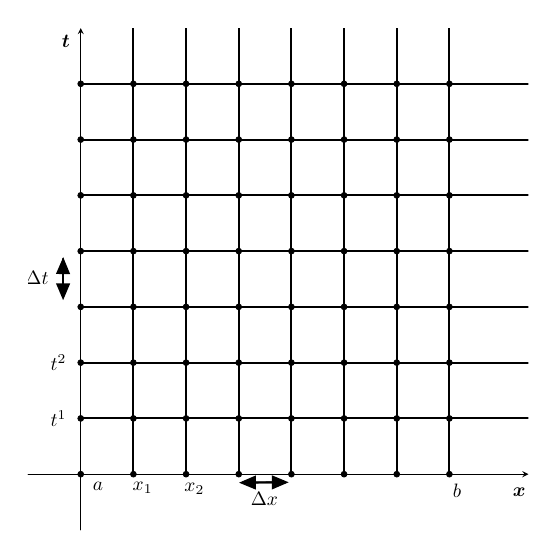
\begin{tikzpicture}[scale=0.7pt,line cap=round,line join=round,>=triangle  45,x=0.9555555555555555cm,y=1.011764705882353cm]
        \begin{axis}[
        x=0.9555555555555555cm,y=1.011764705882353cm,
        axis lines=middle,
        xmin=-1,
        xmax=8.5,
        ymin=-1,
        ymax=8.0,
        xtick={-0.0},
        ytick={-0.0},]
        \clip(-1.0,-1.0) rectangle (8.5,8.5);
        \draw (0.1,-0.01492590769987644) node[anchor=north west] {$a$};
        \draw (6.936006015235138,-0.04625816247894026) node[anchor=north west] {$b$};
        \draw (-1.18,3.765832835640491) node[anchor=north west] {$\Delta t$};
        \draw (3.1,-0.20291943637425935) node[anchor=north west] {$\Delta x$};
        \draw (0.8575485880967675,-0.01492590769987644) node[anchor=north west] {$x_1$};
        \draw (1.839292571174099,-0.03581407755258566) node[anchor=north west] {$x_2$};
        \draw (-0.7,1.2592524533153857) node[anchor=north west] {$t^1$};
        \draw (-0.7,2.2723286911717824) node[anchor=north west] {$t^2$};
        \draw (8.074411272207788,-0.12981084188977712) node[anchor=north west] {$\boldsymbol{x}$};
        \draw (-0.49,8) node[anchor=north west] {$\boldsymbol{t}$};
        \draw [->,line width=1.pt] (-0.3346034577059823,3.8604740672051325) -- (-0.3346034577059823,3.1204740672051328);
        \draw [->,line width=1.pt] (-0.3346034577059823,3.7017839952482134) -- (-0.3329059840463152,3.8906629755388313);
        \draw [->,line width=1.pt] (3.121531540966689,-0.14907205546295046) -- (3.948030184929092,-0.14559937208495718);
        \draw [->,line width=1.pt] (3.823001199491475,-0.1461247039565438) -- (3.0069329894929098,-0.15254473884094374);
        \draw [line width=1.pt] (1.,0.) -- (1.,8.);
        \draw [line width=1.pt] (2.,0.) -- (2.,8.);
        \draw [line width=1.pt] (3.,0.) -- (3.,8.);
        \draw [line width=1.pt] (4.,0.) -- (4.,8.);
        \draw [line width=1.pt] (5.,0.) -- (5.,8.);
        \draw [line width=1.pt] (6.,0.) -- (6.,8.);
        \draw [line width=1.pt] (7.,0.) -- (7.,8.);
        \draw [line width=1.pt,domain=0.0:8.5] plot(\x,{(--7.-0.*\x)/7.});
        \draw [line width=1.pt,domain=0.0:8.5] plot(\x,{(--4.-0.*\x)/2.});
        \draw [line width=1.pt,domain=0.0:8.5] plot(\x,{(--3.-0.*\x)/1.});
        \draw [line width=1.pt,domain=0.0:8.5] plot(\x,{(--4.-0.*\x)/1.});
        \draw [line width=1.pt,domain=0.0:8.5] plot(\x,{(--5.-0.*\x)/1.});
        \draw [line width=1.pt,domain=0.0:8.5] plot(\x,{(--6.-0.*\x)/1.});
        \draw [line width=1.pt,domain=0.0:8.5] plot(\x,{(--7.-0.*\x)/1.});
        \begin{scriptsize}
        \draw [fill=black] (1.,0.) circle (1.5pt);
        \draw [fill=black] (2.,0.) circle (1.5pt);
        \draw [fill=black] (3.,0.) circle (1.5pt);
        \draw [fill=black] (4.,0.) circle (1.5pt);
        \draw [fill=black] (5.,0.) circle (1.5pt);
        \draw [fill=black] (6.,0.) circle (1.5pt);
        \draw [fill=black] (7.,0.) circle (1.5pt);
        \draw [fill=black] (0.,0.) circle (1.5pt);
        \draw [fill=black] (0.,1.) circle (1.5pt);
        \draw [fill=black] (0.,2.) circle (1.5pt);
        \draw [fill=black] (0.,3.) circle (1.5pt);
        \draw [fill=black] (0.,4.) circle (1.5pt);
        \draw [fill=black] (0.,5.) circle (1.5pt);
        \draw [fill=black] (0.,6.) circle (1.5pt);
        \draw [fill=black] (0.,7.) circle (1.5pt);
        \draw [fill=black] (1.,1.) circle (1.5pt);
        \draw [fill=black] (1.,2.) circle (1.5pt);
        \draw [fill=black] (1.,3.) circle (1.5pt);
        \draw [fill=black] (1.,4.) circle (1.5pt);
        \draw [fill=black] (1.,5.) circle (1.5pt);
        \draw [fill=black] (1.,6.) circle (1.5pt);
        \draw [fill=black] (1.,7.) circle (1.5pt);
        \draw [fill=black] (2.,1.) circle (1.5pt);
        \draw [fill=black] (3.,1.) circle (1.5pt);
        \draw [fill=black] (4.,1.) circle (1.5pt);
        \draw [fill=black] (5.,1.) circle (1.5pt);
        \draw [fill=black] (6.,1.) circle (1.5pt);
        \draw [fill=black] (7.,1.) circle (1.5pt);
        \draw [fill=black] (2.,2.) circle (1.5pt);
        \draw [fill=black] (3.,2.) circle (1.5pt);
        \draw [fill=black] (4.,2.) circle (1.5pt);
        \draw [fill=black] (2.,3.) circle (1.5pt);
        \draw [fill=black] (2.,4.) circle (1.5pt);
        \draw [fill=black] (2.,5.) circle (1.5pt);
        \draw [fill=black] (2.,6.) circle (1.5pt);
        \draw [fill=black] (2.,7.) circle (1.5pt);
        \draw [fill=black] (3.,3.) circle (1.5pt);
        \draw [fill=black] (3.,4.) circle (1.5pt);
        \draw [fill=black] (3.,5.) circle (1.5pt);
        \draw [fill=black] (3.,6.) circle (1.5pt);
        \draw [fill=black] (3.,7.) circle (1.5pt);
        \draw [fill=black] (4.,3.) circle (1.5pt);
        \draw [fill=black] (4.,4.) circle (1.5pt);
        \draw [fill=black] (4.,5.) circle (1.5pt);
        \draw [fill=black] (4.,6.) circle (1.5pt);
        \draw [fill=black] (4.,7.) circle (1.5pt);
        \draw [fill=black] (5.,2.) circle (1.5pt);
        \draw [fill=black] (5.,3.) circle (1.5pt);
        \draw [fill=black] (5.,4.) circle (1.5pt);
        \draw [fill=black] (5.,5.) circle (1.5pt);
        \draw [fill=black] (5.,6.) circle (1.5pt);
        \draw [fill=black] (5.,7.) circle (1.5pt);
        \draw [fill=black] (6.,2.) circle (1.5pt);
        \draw [fill=black] (6.,3.) circle (1.5pt);
        \draw [fill=black] (6.,4.) circle (1.5pt);
        \draw [fill=black] (6.,5.) circle (1.5pt);
        \draw [fill=black] (6.,6.) circle (1.5pt);
        \draw [fill=black] (6.,7.) circle (1.5pt);
        \draw [fill=black] (7.,2.) circle (1.5pt);
        \draw [fill=black] (7.,3.) circle (1.5pt);
        \draw [fill=black] (7.,4.) circle (1.5pt);
        \draw [fill=black] (7.,5.) circle (1.5pt);
        \draw [fill=black] (7.,6.) circle (1.5pt);
        \draw [fill=black] (7.,7.) circle (1.5pt);
        \end{scriptsize}
        \end{axis}
        \end{tikzpicture}
    %\caption{}
    %\label{fig:my_label}
\end{figure}

\-\\\underline{Idea}: We'll impose $U_t(x_i,t^n) - U_{xx}(x_i,t^n) = f(x_i,t^n)$

\newpage

\subsubsection{Numerical derivatives}

\definecolor{qqwwzz}{rgb}{0.,0.4,0.6}

\begin{figure}[h]
    \centering
    \begin{tikzpicture}[line cap=round,line join=round,>=triangle 45,x=1.0cm,y=1.0cm]
    \begin{axis}[
    x=1.0cm,y=1.0cm,
    axis lines=middle,
    xmin=9.0,
    xmax=19.0,
    ymin=-1.0,
    ymax=7.0,
    xtick={0.0},
    ytick={0.0},y axis line style={draw = none}]
    \clip(9.,-1.) rectangle (19.,7.);
    \draw[line width=1.pt, smooth,samples=100,domain=0.0:0.11] plot[parametric] function{37.06*t**(3.0)+0.0*t**(2.0)+5.7*t+9.8,-38.54*t**(3.0)+0.0*t**(2.0)+7.51*t+3.02};
    \draw[line width=1.pt, smooth,samples=100,domain=0.11:0.15] plot[parametric] function{-52.47*t**(3.0)+28.91*t**(2.0)+2.59*t+9.91,39.61*t**(3.0)-25.24*t**(2.0)+10.22*t+2.92};
    \draw[line width=1.pt, smooth,samples=100,domain=0.15:0.24] plot[parametric] function{1.47*t**(3.0)+4.08*t**(2.0)+6.4*t+9.72,-18.89*t**(3.0)+1.69*t**(2.0)+6.09*t+3.13};
    \draw[line width=1.pt, smooth,samples=100,domain=0.24:0.3] plot[parametric] function{-13.11*t**(3.0)+14.44*t**(2.0)+3.95*t+9.91,9.63*t**(3.0)-18.57*t**(2.0)+10.89*t+2.76};
    \draw[line width=1.pt, smooth,samples=100,domain=0.3:0.35] plot[parametric] function{-7.62*t**(3.0)+9.58*t**(2.0)+5.38*t+9.77,-31.65*t**(3.0)+18.04*t**(2.0)+0.07*t+3.82};
    \draw[line width=1.pt, smooth,samples=100,domain=0.35:0.41] plot[parametric] function{-10.98*t**(3.0)+13.12*t**(2.0)+4.13*t+9.92,72.27*t**(3.0)-91.76*t**(2.0)+38.74*t-0.72};
    \draw[line width=1.pt, smooth,samples=100,domain=0.41:0.49] plot[parametric] function{3.59*t**(3.0)-4.8*t**(2.0)+11.48*t+8.91,47.73*t**(3.0)-61.58*t**(2.0)+26.37*t+0.97};
    \draw[line width=1.pt, smooth,samples=100,domain=0.49:0.57] plot[parametric] function{-20.86*t**(3.0)+30.92*t**(2.0)-5.91*t+11.73,40.31*t**(3.0)-50.75*t**(2.0)+21.09*t+1.83};
    \draw[line width=1.pt, smooth,samples=100,domain=0.57:0.62] plot[parametric] function{-10.43*t**(3.0)+13.18*t**(2.0)+4.14*t+9.84,-36.6*t**(3.0)+80.04*t**(2.0)-53.05*t+15.84};
    \draw[line width=1.pt, smooth,samples=100,domain=0.62:0.7] plot[parametric] function{28.35*t**(3.0)-59.13*t**(2.0)+49.1*t+0.52,-54.92*t**(3.0)+114.21*t**(2.0)-74.29*t+20.24};
    \draw[line width=1.pt, smooth,samples=100,domain=0.7:0.77] plot[parametric] function{-7.01*t**(3.0)+14.63*t**(2.0)-2.2*t+12.41,14.24*t**(3.0)-30.06*t**(2.0)+26.04*t-3.02};
    \draw[line width=1.pt, smooth,samples=100,domain=0.77:0.85] plot[parametric] function{36.51*t**(3.0)-85.69*t**(2.0)+74.89*t-7.34,-63.54*t**(3.0)+149.23*t**(2.0)-111.73*t+32.27};
    \draw[line width=1.pt, smooth,samples=100,domain=0.85:0.92] plot[parametric] function{-17.36*t**(3.0)+51.06*t**(2.0)-40.83*t+25.3,-8.72*t**(3.0)+10.06*t**(2.0)+6.03*t-0.95};
    \draw [line width=1.pt,dotted] (14.,0.)-- (13.99722993459645,4.732881120180119);
    \draw [line width=1.pt, >=latex, <->] (10.2,0.36)-- (13.6,0.36);
    \draw [line width=1.pt, >=latex, <->] (14.38,0.34)-- (17.88,0.34);
    \draw (11.76,1.06) node[anchor=north west] {$h$};
    \draw (15.9,1.04) node[anchor=north west] {$h$};
    \draw (9.52,0.) node[anchor=north west] {$x_{i-1}$};
    \draw (17.94,-0.04) node[anchor=north west] {$x_{i+1}$};
    \draw (13.84,0.) node[anchor=north west] {$x_{i}$};
    \draw (17.5,6.6) node[anchor=north west] {$f$};
    \draw (13,5.58) node[anchor=north west] {$f_i = f(x_i)$};
    \begin{scriptsize}
    \draw [color=qqwwzz] (14.,0.)-- ++(-1.5pt,0 pt) -- ++(3.0pt,0 pt) ++(-1.5pt,-1.5pt) -- ++(0 pt,3.0pt);
    \draw [fill=qqwwzz] (13.99722993459645,4.732881120180119) circle (1.5pt);
    \draw [color=black] (9.82,0.)-- ++(-1.5pt,0 pt) -- ++(3.0pt,0 pt) ++(-1.5pt,-1.5pt) -- ++(0 pt,3.0pt);
    \draw [color=black] (18.18,0.)-- ++(-1.5pt,0 pt) -- ++(3.0pt,0 pt) ++(-1.5pt,-1.5pt) -- ++(0 pt,3.0pt);
    \draw [fill=black,shift={(10.2,0.36)},rotate=90] (0,0) ++(0 pt,2.25pt) -- ++(1.9485571585149868pt,-3.375pt)--++(-3.8971143170299736pt,0 pt) -- ++(1.9485571585149868pt,3.375pt);
    \draw [fill=black,shift={(13.6,0.36)},rotate=270] (0,0) ++(0 pt,2.25pt) -- ++(1.9485571585149868pt,-3.375pt)--++(-3.8971143170299736pt,0 pt) -- ++(1.9485571585149868pt,3.375pt);
    \draw [fill=black,shift={(14.38,0.34)},rotate=90] (0,0) ++(0 pt,2.25pt) -- ++(1.9485571585149868pt,-3.375pt)--++(-3.8971143170299736pt,0 pt) -- ++(1.9485571585149868pt,3.375pt);
    \draw [fill=black,shift={(17.88,0.34)},rotate=270] (0,0) ++(0 pt,2.25pt) -- ++(1.9485571585149868pt,-3.375pt)--++(-3.8971143170299736pt,0 pt) -- ++(1.9485571585149868pt,3.375pt);
    \end{scriptsize}
    \end{axis}
    \end{tikzpicture}
    %\caption{}
    %\label{fig:my_label}
\end{figure}


\newpage
\section{Numerical Solution of PDEs with the Finite Difference Method}
\newpage
\section{Introduction to Boundary Value Problems}
\newpage
\section{Quality Control of Solutions}

\end{document}

